\documentclass[twoside]{book}

% Packages required by doxygen
\usepackage{fixltx2e}
\usepackage{calc}
\usepackage{doxygen}
\usepackage[export]{adjustbox} % also loads graphicx
\usepackage{graphicx}
\usepackage[utf8]{inputenc}
\usepackage{makeidx}
\usepackage{multicol}
\usepackage{multirow}
\PassOptionsToPackage{warn}{textcomp}
\usepackage{textcomp}
\usepackage[nointegrals]{wasysym}
\usepackage[table]{xcolor}

% NLS support packages
\usepackage[brazil]{babel}
% Font selection
\usepackage[T1]{fontenc}
\usepackage[scaled=.90]{helvet}
\usepackage{courier}
\usepackage{amssymb}
\usepackage{sectsty}
\renewcommand{\familydefault}{\sfdefault}
\allsectionsfont{%
  \fontseries{bc}\selectfont%
  \color{darkgray}%
}
\renewcommand{\DoxyLabelFont}{%
  \fontseries{bc}\selectfont%
  \color{darkgray}%
}
\newcommand{\+}{\discretionary{\mbox{\scriptsize$\hookleftarrow$}}{}{}}

% Page & text layout
\usepackage{geometry}
\geometry{%
  a4paper,%
  top=2.5cm,%
  bottom=2.5cm,%
  left=2.5cm,%
  right=2.5cm%
}
\tolerance=750
\hfuzz=15pt
\hbadness=750
\setlength{\emergencystretch}{15pt}
\setlength{\parindent}{0cm}
\setlength{\parskip}{3ex plus 2ex minus 2ex}
\makeatletter
\renewcommand{\paragraph}{%
  \@startsection{paragraph}{4}{0ex}{-1.0ex}{1.0ex}{%
    \normalfont\normalsize\bfseries\SS@parafont%
  }%
}
\renewcommand{\subparagraph}{%
  \@startsection{subparagraph}{5}{0ex}{-1.0ex}{1.0ex}{%
    \normalfont\normalsize\bfseries\SS@subparafont%
  }%
}
\makeatother

% Headers & footers
\usepackage{fancyhdr}
\pagestyle{fancyplain}
\fancyhead[LE]{\fancyplain{}{\bfseries\thepage}}
\fancyhead[CE]{\fancyplain{}{}}
\fancyhead[RE]{\fancyplain{}{\bfseries\leftmark}}
\fancyhead[LO]{\fancyplain{}{\bfseries\rightmark}}
\fancyhead[CO]{\fancyplain{}{}}
\fancyhead[RO]{\fancyplain{}{\bfseries\thepage}}
\fancyfoot[LE]{\fancyplain{}{}}
\fancyfoot[CE]{\fancyplain{}{}}
\fancyfoot[RE]{\fancyplain{}{\bfseries\scriptsize Gerado por Doxygen }}
\fancyfoot[LO]{\fancyplain{}{\bfseries\scriptsize Gerado por Doxygen }}
\fancyfoot[CO]{\fancyplain{}{}}
\fancyfoot[RO]{\fancyplain{}{}}
\renewcommand{\footrulewidth}{0.4pt}
\renewcommand{\chaptermark}[1]{%
  \markboth{#1}{}%
}
\renewcommand{\sectionmark}[1]{%
  \markright{\thesection\ #1}%
}

% Indices & bibliography
\usepackage{natbib}
\usepackage[titles]{tocloft}
\setcounter{tocdepth}{3}
\setcounter{secnumdepth}{5}
\makeindex

% Hyperlinks (required, but should be loaded last)
\usepackage{ifpdf}
\ifpdf
  \usepackage[pdftex,pagebackref=true]{hyperref}
\else
  \usepackage[ps2pdf,pagebackref=true]{hyperref}
\fi
\hypersetup{%
  colorlinks=true,%
  linkcolor=blue,%
  citecolor=blue,%
  unicode%
}

% Custom commands
\newcommand{\clearemptydoublepage}{%
  \newpage{\pagestyle{empty}\cleardoublepage}%
}

\usepackage{caption}
\captionsetup{labelsep=space,justification=centering,font={bf},singlelinecheck=off,skip=4pt,position=top}

%===== C O N T E N T S =====

\begin{document}

% Titlepage & ToC
\hypersetup{pageanchor=false,
             bookmarksnumbered=true,
             pdfencoding=unicode
            }
\pagenumbering{alph}
\begin{titlepage}
\vspace*{7cm}
\begin{center}%
{\Large Projeto de Polígonos -\/ Programação Avançada }\\
\vspace*{1cm}
{\large Gerado por Doxygen 1.8.13}\\
\end{center}
\end{titlepage}
\clearemptydoublepage
\pagenumbering{roman}
\tableofcontents
\clearemptydoublepage
\pagenumbering{arabic}
\hypersetup{pageanchor=true}

%--- Begin generated contents ---
\chapter{Projeto 1 -\/ Tratamento de polígonos}
\label{index}\hypertarget{index}{}\hypertarget{index_intro}{}\section{Introdução}\label{index_intro}
Este projeto é um instrumento avaliativo da segunda unidade da turma D\+C\+A1202 -\/ Programação Avançada, lecionada pelo professor Agostinho Brito. O projeto é capaz de armazenar e realizar operações com polígonos formados por conjuntos de pontos em duas dimensões.

Está previsto no projeto a criação de três classes, referenciadas a seguir\+:

\mbox{\hyperlink{classPonto}{Ponto}}

\mbox{\hyperlink{classPoligono}{Poligono}}

\mbox{\hyperlink{classRetangulo}{Retangulo}}\hypertarget{index_componente}{}\section{Componente}\label{index_componente}
\hypertarget{index_nome}{}\subsection{Beatriz Soares de Souza -\/ 2016021417}\label{index_nome}

\chapter{Program\+Avanc}
\label{md_README}
\Hypertarget{md_README}
\input{md_README}
\chapter{Índice Hierárquico}
\section{Hierarquia de Classes}
Esta lista de hierarquias está parcialmente ordenada (ordem alfabética)\+:\begin{DoxyCompactList}
\item \contentsline{section}{Poligono}{\pageref{classPoligono}}{}
\begin{DoxyCompactList}
\item \contentsline{section}{Retangulo}{\pageref{classRetangulo}}{}
\item \contentsline{section}{Retangulo}{\pageref{classRetangulo}}{}
\end{DoxyCompactList}
\item \contentsline{section}{Ponto}{\pageref{classPonto}}{}
\end{DoxyCompactList}

\chapter{Índice dos Componentes}
\section{Class List}
Here are the classes, structs, unions and interfaces with brief descriptions\+:\begin{DoxyCompactList}
\item\contentsline{section}{\mbox{\hyperlink{classPoligono}{Poligono}} \\*A \mbox{\hyperlink{classPoligono}{Poligono}} class }{\pageref{classPoligono}}{}
\item\contentsline{section}{\mbox{\hyperlink{classPonto}{Ponto}} \\*A \mbox{\hyperlink{classPonto}{Ponto}} class }{\pageref{classPonto}}{}
\item\contentsline{section}{\mbox{\hyperlink{classRetangulo}{Retangulo}} }{\pageref{classRetangulo}}{}
\end{DoxyCompactList}

\chapter{Classes}
\hypertarget{classPoligono}{}\section{Poligono Class Reference}
\label{classPoligono}\index{Poligono@{Poligono}}


A \mbox{\hyperlink{classPoligono}{Poligono}} class.  




{\ttfamily \#include $<$poligono.\+h$>$}

Inheritance diagram for Poligono\+:\begin{figure}[H]
\begin{center}
\leavevmode
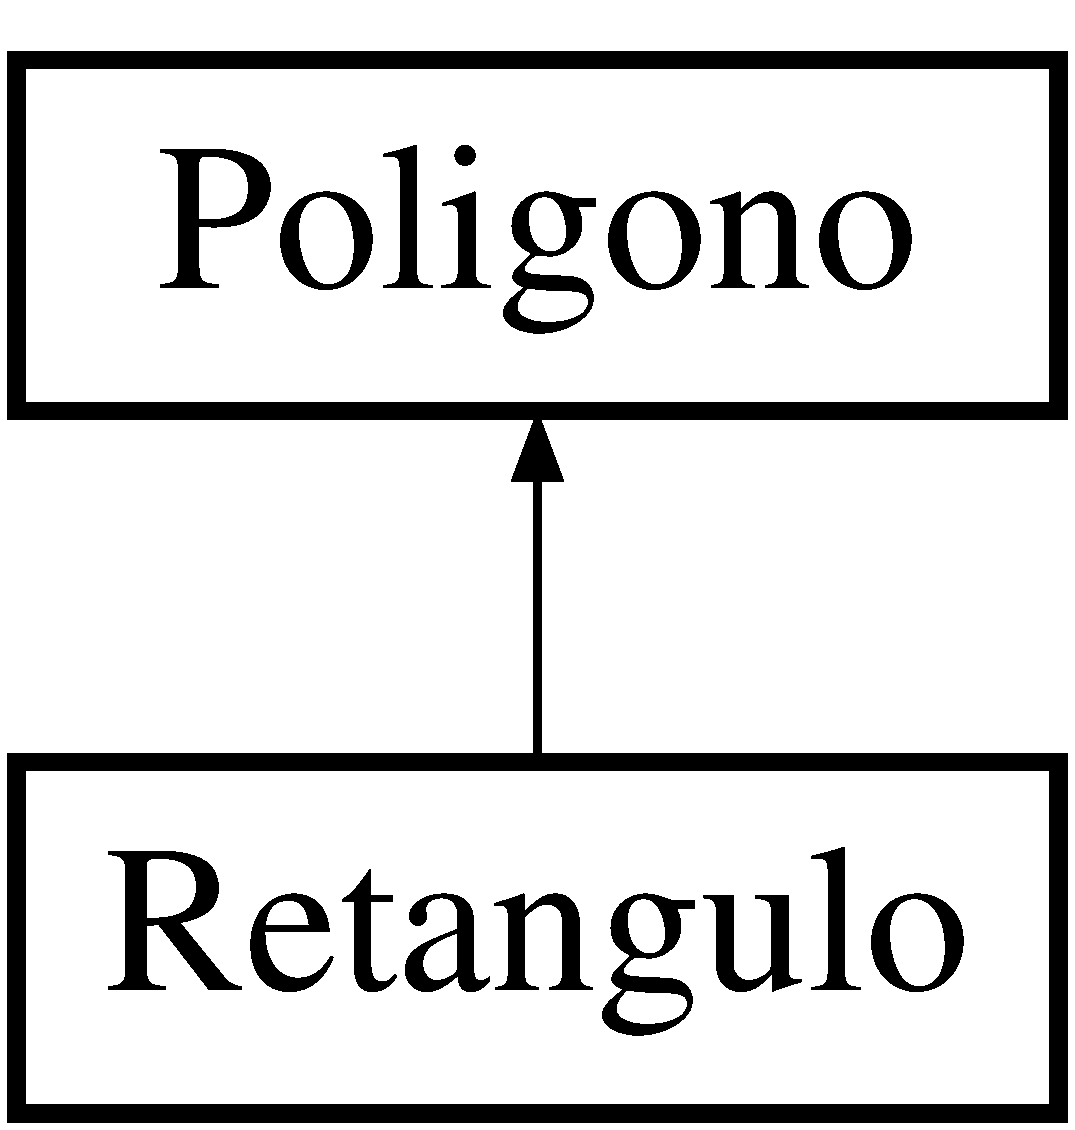
\includegraphics[height=2.000000cm]{classPoligono}
\end{center}
\end{figure}
\subsection*{Public Member Functions}
\begin{DoxyCompactItemize}
\item 
\mbox{\Hypertarget{classPoligono_a9311a9a1496878c09c8508b3636e2870}\label{classPoligono_a9311a9a1496878c09c8508b3636e2870}} 
\mbox{\hyperlink{classPoligono_a9311a9a1496878c09c8508b3636e2870}{Poligono}} ()
\begin{DoxyCompactList}\small\item\em Construtor da Classe. \end{DoxyCompactList}\item 
void \mbox{\hyperlink{classPoligono_aeaad76667207d96ea0d69c2dfb3bc2a9}{insere\+Vertice}} (float x, float y)
\begin{DoxyCompactList}\small\item\em Método que insere no vetor \textquotesingle{}vertices\textquotesingle{} um novo ponto, com as coordenadas passadas no argumento. \end{DoxyCompactList}\item 
int \mbox{\hyperlink{classPoligono_ae2c1c915b4a72104724d1302138e7caa}{qtd\+Vertices}} ()
\begin{DoxyCompactList}\small\item\em Método que retorna a quantidade de vertices que o polígono possui. \end{DoxyCompactList}\item 
float \mbox{\hyperlink{classPoligono_ab1a85a090e7442bf3151602b05da9e19}{get\+Area}} ()
\begin{DoxyCompactList}\small\item\em Método que retorna a área do polígono. \end{DoxyCompactList}\item 
void \mbox{\hyperlink{classPoligono_adbf605dfd0419b7301c9be0ec1dbe41b}{translada}} (float a, float b)
\begin{DoxyCompactList}\small\item\em Método que translada o polígono, ponto a ponto, de acordo com os argumentos passados. \end{DoxyCompactList}\item 
void \mbox{\hyperlink{classPoligono_a937c0e2bec60140fcc7b7bde5d64d339}{rotaciona}} (float teta)
\begin{DoxyCompactList}\small\item\em Método que rotaciona o polígono, a partir de um ponto, em teta graus. \end{DoxyCompactList}\item 
\mbox{\Hypertarget{classPoligono_aeaad76667207d96ea0d69c2dfb3bc2a9}\label{classPoligono_aeaad76667207d96ea0d69c2dfb3bc2a9}} 
void {\bfseries insere\+Vertice} (float x, float y)
\item 
\mbox{\Hypertarget{classPoligono_ae2c1c915b4a72104724d1302138e7caa}\label{classPoligono_ae2c1c915b4a72104724d1302138e7caa}} 
int {\bfseries qtd\+Vertices} ()
\item 
\mbox{\Hypertarget{classPoligono_ab1a85a090e7442bf3151602b05da9e19}\label{classPoligono_ab1a85a090e7442bf3151602b05da9e19}} 
float {\bfseries get\+Area} ()
\item 
\mbox{\Hypertarget{classPoligono_adbf605dfd0419b7301c9be0ec1dbe41b}\label{classPoligono_adbf605dfd0419b7301c9be0ec1dbe41b}} 
void {\bfseries translada} (float a, float b)
\item 
\mbox{\Hypertarget{classPoligono_a93da79ac2b0cfd723c4c041f2fe1190c}\label{classPoligono_a93da79ac2b0cfd723c4c041f2fe1190c}} 
void {\bfseries rotaciona} (float teta, float \+\_\+x, float \+\_\+y)
\end{DoxyCompactItemize}


\subsection{Detailed Description}
A \mbox{\hyperlink{classPoligono}{Poligono}} class. 

A more elaborate class description. 

\subsection{Member Function Documentation}
\mbox{\Hypertarget{classPoligono_ab1a85a090e7442bf3151602b05da9e19}\label{classPoligono_ab1a85a090e7442bf3151602b05da9e19}} 
\index{Poligono@{Poligono}!get\+Area@{get\+Area}}
\index{get\+Area@{get\+Area}!Poligono@{Poligono}}
\subsubsection{\texorpdfstring{get\+Area()}{getArea()}}
{\footnotesize\ttfamily float Poligono\+::get\+Area (\begin{DoxyParamCaption}{ }\end{DoxyParamCaption})}



Método que retorna a área do polígono. 

\begin{DoxyReturn}{Returns}
um float indicando a área do polígono. 
\end{DoxyReturn}
\mbox{\Hypertarget{classPoligono_aeaad76667207d96ea0d69c2dfb3bc2a9}\label{classPoligono_aeaad76667207d96ea0d69c2dfb3bc2a9}} 
\index{Poligono@{Poligono}!insere\+Vertice@{insere\+Vertice}}
\index{insere\+Vertice@{insere\+Vertice}!Poligono@{Poligono}}
\subsubsection{\texorpdfstring{insere\+Vertice()}{insereVertice()}}
{\footnotesize\ttfamily void Poligono\+::insere\+Vertice (\begin{DoxyParamCaption}\item[{float}]{x,  }\item[{float}]{y }\end{DoxyParamCaption})}



Método que insere no vetor \textquotesingle{}vertices\textquotesingle{} um novo ponto, com as coordenadas passadas no argumento. 


\begin{DoxyParams}{Parameters}
{\em x} & argumento float. \\
\hline
{\em y} & argumento float. \\
\hline
\end{DoxyParams}
\mbox{\Hypertarget{classPoligono_ae2c1c915b4a72104724d1302138e7caa}\label{classPoligono_ae2c1c915b4a72104724d1302138e7caa}} 
\index{Poligono@{Poligono}!qtd\+Vertices@{qtd\+Vertices}}
\index{qtd\+Vertices@{qtd\+Vertices}!Poligono@{Poligono}}
\subsubsection{\texorpdfstring{qtd\+Vertices()}{qtdVertices()}}
{\footnotesize\ttfamily int Poligono\+::qtd\+Vertices (\begin{DoxyParamCaption}{ }\end{DoxyParamCaption})}



Método que retorna a quantidade de vertices que o polígono possui. 

\begin{DoxyReturn}{Returns}
um inteiro indicando a quantidade de vértices do polígono. 
\end{DoxyReturn}
\mbox{\Hypertarget{classPoligono_a937c0e2bec60140fcc7b7bde5d64d339}\label{classPoligono_a937c0e2bec60140fcc7b7bde5d64d339}} 
\index{Poligono@{Poligono}!rotaciona@{rotaciona}}
\index{rotaciona@{rotaciona}!Poligono@{Poligono}}
\subsubsection{\texorpdfstring{rotaciona()}{rotaciona()}}
{\footnotesize\ttfamily void Poligono\+::rotaciona (\begin{DoxyParamCaption}\item[{float}]{teta }\end{DoxyParamCaption})}



Método que rotaciona o polígono, a partir de um ponto, em teta graus. 


\begin{DoxyParams}{Parameters}
{\em teta} & float indicará o ângulo em que o poligono será rotacionado. \\
\hline
{\em \+\_\+x} & float que indica a coordenada X do ponto de referência da rotação. \\
\hline
{\em \+\_\+y} & float que indica a coordenada Y do ponto de referência da rotação. \\
\hline
\end{DoxyParams}
\mbox{\Hypertarget{classPoligono_adbf605dfd0419b7301c9be0ec1dbe41b}\label{classPoligono_adbf605dfd0419b7301c9be0ec1dbe41b}} 
\index{Poligono@{Poligono}!translada@{translada}}
\index{translada@{translada}!Poligono@{Poligono}}
\subsubsection{\texorpdfstring{translada()}{translada()}}
{\footnotesize\ttfamily void Poligono\+::translada (\begin{DoxyParamCaption}\item[{float}]{a,  }\item[{float}]{b }\end{DoxyParamCaption})}



Método que translada o polígono, ponto a ponto, de acordo com os argumentos passados. 


\begin{DoxyParams}{Parameters}
{\em a} & float que será somado com as coordenadas X dos pontos. \\
\hline
{\em b} & float que será somado com as coordenadas Y dos pontos. \\
\hline
\end{DoxyParams}


The documentation for this class was generated from the following files\+:\begin{DoxyCompactItemize}
\item 
poligono.\+h\item 
projeto.\+cpp\item 
poligono.\+cpp\end{DoxyCompactItemize}

\hypertarget{classPonto}{}\section{Ponto Class Reference}
\label{classPonto}\index{Ponto@{Ponto}}


A \mbox{\hyperlink{classPonto}{Ponto}} class.  


\subsection*{Public Member Functions}
\begin{DoxyCompactItemize}
\item 
\mbox{\Hypertarget{classPonto_a22129ad4dbf8019c479021d70a9f6774}\label{classPonto_a22129ad4dbf8019c479021d70a9f6774}} 
void {\bfseries setX} (float \+\_\+x)
\item 
\mbox{\Hypertarget{classPonto_a2d9e5b9fade9d3f3f21122a2dc2f5e11}\label{classPonto_a2d9e5b9fade9d3f3f21122a2dc2f5e11}} 
void {\bfseries setY} (float \+\_\+y)
\item 
\mbox{\Hypertarget{classPonto_a827488219a7da184d440f687cec49ce6}\label{classPonto_a827488219a7da184d440f687cec49ce6}} 
void {\bfseries set\+XY} (float \+\_\+x, float \+\_\+y)
\item 
\mbox{\Hypertarget{classPonto_ae4823d6ee26ff3448ee403d26a3c6d2f}\label{classPonto_ae4823d6ee26ff3448ee403d26a3c6d2f}} 
float {\bfseries getX} ()
\item 
\mbox{\Hypertarget{classPonto_ab120600953e6544301223b9b05a43ee5}\label{classPonto_ab120600953e6544301223b9b05a43ee5}} 
float {\bfseries getY} ()
\item 
\mbox{\Hypertarget{classPonto_abb68d6122278de262e8ed1c70714e3d9}\label{classPonto_abb68d6122278de262e8ed1c70714e3d9}} 
\mbox{\hyperlink{classPonto}{Ponto}} {\bfseries add} (\mbox{\hyperlink{classPonto}{Ponto}} p1)
\item 
\mbox{\Hypertarget{classPonto_a8404fcad0fca2ce768ab9e1550f5d3a0}\label{classPonto_a8404fcad0fca2ce768ab9e1550f5d3a0}} 
\mbox{\hyperlink{classPonto}{Ponto}} {\bfseries sub} (\mbox{\hyperlink{classPonto}{Ponto}} p1)
\item 
\mbox{\Hypertarget{classPonto_a9b0ddbdddd05edbc4d45ef0671a628c6}\label{classPonto_a9b0ddbdddd05edbc4d45ef0671a628c6}} 
float {\bfseries norma} ()
\item 
\mbox{\Hypertarget{classPonto_a96a4395204ec010814e67d20705e630f}\label{classPonto_a96a4395204ec010814e67d20705e630f}} 
void {\bfseries translada} (float a, float b)
\item 
\mbox{\Hypertarget{classPonto_a84758d453e38f237bdf860b6435e9def}\label{classPonto_a84758d453e38f237bdf860b6435e9def}} 
void {\bfseries imprime} ()
\item 
void \mbox{\hyperlink{classPonto_a22129ad4dbf8019c479021d70a9f6774}{setX}} (float \+\_\+x)
\begin{DoxyCompactList}\small\item\em Método que seta um valor para a coordenada X do ponto. \end{DoxyCompactList}\item 
void \mbox{\hyperlink{classPonto_a2d9e5b9fade9d3f3f21122a2dc2f5e11}{setY}} (float \+\_\+y)
\begin{DoxyCompactList}\small\item\em Método que seta um valor para a coordenada Y do ponto. \end{DoxyCompactList}\item 
void \mbox{\hyperlink{classPonto_a827488219a7da184d440f687cec49ce6}{set\+XY}} (float \+\_\+x, float \+\_\+y)
\begin{DoxyCompactList}\small\item\em Método que seta os valores para as coordenadas X e Y do ponto. \end{DoxyCompactList}\item 
float \mbox{\hyperlink{classPonto_ae4823d6ee26ff3448ee403d26a3c6d2f}{getX}} ()
\begin{DoxyCompactList}\small\item\em Método que retorna a coordenada X do ponto. \end{DoxyCompactList}\item 
float \mbox{\hyperlink{classPonto_ab120600953e6544301223b9b05a43ee5}{getY}} ()
\begin{DoxyCompactList}\small\item\em Método que retorna a coordenada Y do ponto. \end{DoxyCompactList}\item 
\mbox{\hyperlink{classPonto}{Ponto}} \mbox{\hyperlink{classPonto_abb68d6122278de262e8ed1c70714e3d9}{add}} (\mbox{\hyperlink{classPonto}{Ponto}} p1)
\begin{DoxyCompactList}\small\item\em Método que soma as coordenadas X e Y com as coordenadas de um ponto passado no argumento. \end{DoxyCompactList}\item 
\mbox{\hyperlink{classPonto}{Ponto}} \mbox{\hyperlink{classPonto_a8404fcad0fca2ce768ab9e1550f5d3a0}{sub}} (\mbox{\hyperlink{classPonto}{Ponto}} p1)
\begin{DoxyCompactList}\small\item\em Método que subtrai as coordenadas X e Y das coordenadas de um ponto passado no argumento. \end{DoxyCompactList}\item 
float \mbox{\hyperlink{classPonto_a9b0ddbdddd05edbc4d45ef0671a628c6}{norma}} ()
\begin{DoxyCompactList}\small\item\em Método que retorna o módulo de um vetor partindo da origem e indo até o ponto. \end{DoxyCompactList}\item 
void \mbox{\hyperlink{classPonto_a96a4395204ec010814e67d20705e630f}{translada}} (float a, float b)
\begin{DoxyCompactList}\small\item\em Método que recebe dois valores e adiciona o primeiro ao X e o segundo ao Y, transladando o ponto. \end{DoxyCompactList}\item 
\mbox{\Hypertarget{classPonto_a84758d453e38f237bdf860b6435e9def}\label{classPonto_a84758d453e38f237bdf860b6435e9def}} 
void \mbox{\hyperlink{classPonto_a84758d453e38f237bdf860b6435e9def}{imprime}} ()
\begin{DoxyCompactList}\small\item\em Método que imprime as coordenadas do ponto, no formato (x,y). \end{DoxyCompactList}\end{DoxyCompactItemize}


\subsection{Detailed Description}
A \mbox{\hyperlink{classPonto}{Ponto}} class. 

A more elaborate class description. 

\subsection{Member Function Documentation}
\mbox{\Hypertarget{classPonto_abb68d6122278de262e8ed1c70714e3d9}\label{classPonto_abb68d6122278de262e8ed1c70714e3d9}} 
\index{Ponto@{Ponto}!add@{add}}
\index{add@{add}!Ponto@{Ponto}}
\subsubsection{\texorpdfstring{add()}{add()}}
{\footnotesize\ttfamily \mbox{\hyperlink{classPonto}{Ponto}} Ponto\+::add (\begin{DoxyParamCaption}\item[{\mbox{\hyperlink{classPonto}{Ponto}}}]{p1 }\end{DoxyParamCaption})\hspace{0.3cm}{\ttfamily [inline]}}



Método que soma as coordenadas X e Y com as coordenadas de um ponto passado no argumento. 


\begin{DoxyParams}{Parameters}
{\em p1} & um argumento do tipo \mbox{\hyperlink{classPonto}{Ponto}}. \\
\hline
\end{DoxyParams}
\begin{DoxyReturn}{Returns}
Um \mbox{\hyperlink{classPonto}{Ponto}} resultante da soma dos dois. 
\end{DoxyReturn}
\mbox{\Hypertarget{classPonto_ae4823d6ee26ff3448ee403d26a3c6d2f}\label{classPonto_ae4823d6ee26ff3448ee403d26a3c6d2f}} 
\index{Ponto@{Ponto}!getX@{getX}}
\index{getX@{getX}!Ponto@{Ponto}}
\subsubsection{\texorpdfstring{get\+X()}{getX()}}
{\footnotesize\ttfamily float Ponto\+::getX (\begin{DoxyParamCaption}{ }\end{DoxyParamCaption})\hspace{0.3cm}{\ttfamily [inline]}}



Método que retorna a coordenada X do ponto. 

\begin{DoxyReturn}{Returns}
Coordenada X (float) 
\end{DoxyReturn}
\mbox{\Hypertarget{classPonto_ab120600953e6544301223b9b05a43ee5}\label{classPonto_ab120600953e6544301223b9b05a43ee5}} 
\index{Ponto@{Ponto}!getY@{getY}}
\index{getY@{getY}!Ponto@{Ponto}}
\subsubsection{\texorpdfstring{get\+Y()}{getY()}}
{\footnotesize\ttfamily float Ponto\+::getY (\begin{DoxyParamCaption}{ }\end{DoxyParamCaption})\hspace{0.3cm}{\ttfamily [inline]}}



Método que retorna a coordenada Y do ponto. 

\begin{DoxyReturn}{Returns}
Coordenada Y (float) 
\end{DoxyReturn}
\mbox{\Hypertarget{classPonto_a9b0ddbdddd05edbc4d45ef0671a628c6}\label{classPonto_a9b0ddbdddd05edbc4d45ef0671a628c6}} 
\index{Ponto@{Ponto}!norma@{norma}}
\index{norma@{norma}!Ponto@{Ponto}}
\subsubsection{\texorpdfstring{norma()}{norma()}}
{\footnotesize\ttfamily float Ponto\+::norma (\begin{DoxyParamCaption}{ }\end{DoxyParamCaption})\hspace{0.3cm}{\ttfamily [inline]}}



Método que retorna o módulo de um vetor partindo da origem e indo até o ponto. 

\begin{DoxyReturn}{Returns}
A norma do vetor da origem ao ponto, do tipo float. 
\end{DoxyReturn}
\mbox{\Hypertarget{classPonto_a22129ad4dbf8019c479021d70a9f6774}\label{classPonto_a22129ad4dbf8019c479021d70a9f6774}} 
\index{Ponto@{Ponto}!setX@{setX}}
\index{setX@{setX}!Ponto@{Ponto}}
\subsubsection{\texorpdfstring{set\+X()}{setX()}}
{\footnotesize\ttfamily void Ponto\+::setX (\begin{DoxyParamCaption}\item[{float}]{\+\_\+x }\end{DoxyParamCaption})\hspace{0.3cm}{\ttfamily [inline]}}



Método que seta um valor para a coordenada X do ponto. 


\begin{DoxyParams}{Parameters}
{\em \+\_\+x} & argumento float. \\
\hline
\end{DoxyParams}
\mbox{\Hypertarget{classPonto_a827488219a7da184d440f687cec49ce6}\label{classPonto_a827488219a7da184d440f687cec49ce6}} 
\index{Ponto@{Ponto}!set\+XY@{set\+XY}}
\index{set\+XY@{set\+XY}!Ponto@{Ponto}}
\subsubsection{\texorpdfstring{set\+X\+Y()}{setXY()}}
{\footnotesize\ttfamily void Ponto\+::set\+XY (\begin{DoxyParamCaption}\item[{float}]{\+\_\+x,  }\item[{float}]{\+\_\+y }\end{DoxyParamCaption})\hspace{0.3cm}{\ttfamily [inline]}}



Método que seta os valores para as coordenadas X e Y do ponto. 


\begin{DoxyParams}{Parameters}
{\em \+\_\+x} & argumento float. \\
\hline
{\em \+\_\+y} & argumento float. \\
\hline
\end{DoxyParams}
\mbox{\Hypertarget{classPonto_a2d9e5b9fade9d3f3f21122a2dc2f5e11}\label{classPonto_a2d9e5b9fade9d3f3f21122a2dc2f5e11}} 
\index{Ponto@{Ponto}!setY@{setY}}
\index{setY@{setY}!Ponto@{Ponto}}
\subsubsection{\texorpdfstring{set\+Y()}{setY()}}
{\footnotesize\ttfamily void Ponto\+::setY (\begin{DoxyParamCaption}\item[{float}]{\+\_\+y }\end{DoxyParamCaption})\hspace{0.3cm}{\ttfamily [inline]}}



Método que seta um valor para a coordenada Y do ponto. 


\begin{DoxyParams}{Parameters}
{\em \+\_\+y} & argumento float. \\
\hline
\end{DoxyParams}
\mbox{\Hypertarget{classPonto_a8404fcad0fca2ce768ab9e1550f5d3a0}\label{classPonto_a8404fcad0fca2ce768ab9e1550f5d3a0}} 
\index{Ponto@{Ponto}!sub@{sub}}
\index{sub@{sub}!Ponto@{Ponto}}
\subsubsection{\texorpdfstring{sub()}{sub()}}
{\footnotesize\ttfamily \mbox{\hyperlink{classPonto}{Ponto}} Ponto\+::sub (\begin{DoxyParamCaption}\item[{\mbox{\hyperlink{classPonto}{Ponto}}}]{p1 }\end{DoxyParamCaption})\hspace{0.3cm}{\ttfamily [inline]}}



Método que subtrai as coordenadas X e Y das coordenadas de um ponto passado no argumento. 


\begin{DoxyParams}{Parameters}
{\em p1} & um argumento do tipo \mbox{\hyperlink{classPonto}{Ponto}}. \\
\hline
\end{DoxyParams}
\begin{DoxyReturn}{Returns}
Um \mbox{\hyperlink{classPonto}{Ponto}} resultante da subtração dos dois. 
\end{DoxyReturn}
\mbox{\Hypertarget{classPonto_a96a4395204ec010814e67d20705e630f}\label{classPonto_a96a4395204ec010814e67d20705e630f}} 
\index{Ponto@{Ponto}!translada@{translada}}
\index{translada@{translada}!Ponto@{Ponto}}
\subsubsection{\texorpdfstring{translada()}{translada()}}
{\footnotesize\ttfamily void Ponto\+::translada (\begin{DoxyParamCaption}\item[{float}]{a,  }\item[{float}]{b }\end{DoxyParamCaption})\hspace{0.3cm}{\ttfamily [inline]}}



Método que recebe dois valores e adiciona o primeiro ao X e o segundo ao Y, transladando o ponto. 


\begin{DoxyParams}{Parameters}
{\em a} & um argumento do tipo float. \\
\hline
{\em b} & um argumento do tipo float. \\
\hline
\end{DoxyParams}


The documentation for this class was generated from the following files\+:\begin{DoxyCompactItemize}
\item 
ponto.\+h\item 
projeto.\+cpp\item 
ponto.\+cpp\end{DoxyCompactItemize}

\hypertarget{classRetangulo}{}\section{Referência da Classe Retangulo}
\label{classRetangulo}\index{Retangulo@{Retangulo}}


Classe \mbox{\hyperlink{classRetangulo}{Retangulo}}.  




{\ttfamily \#include $<$retangulo.\+h$>$}

Diagrama de hierarquia para Retangulo\+:\begin{figure}[H]
\begin{center}
\leavevmode
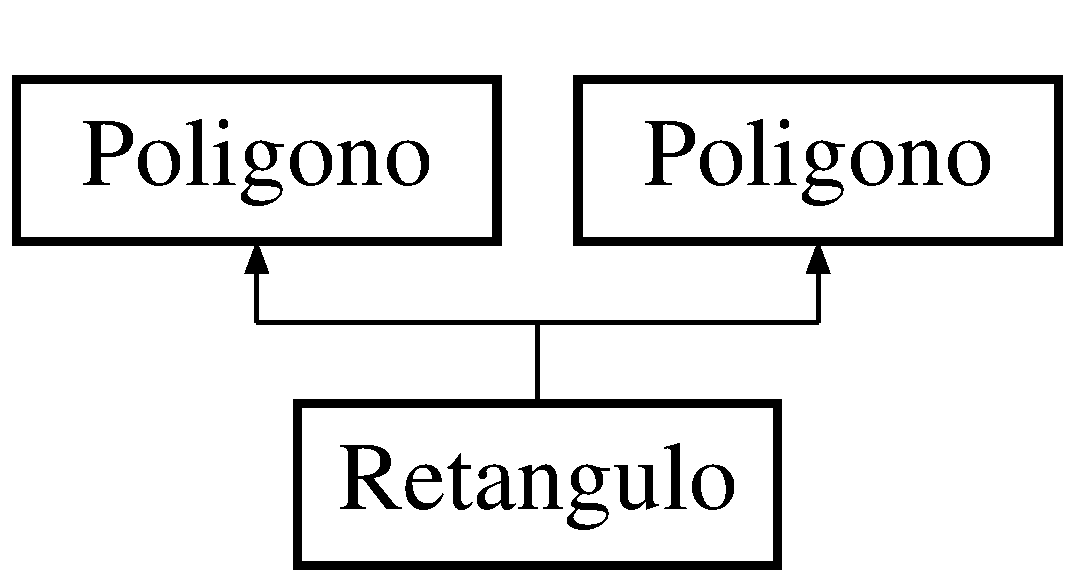
\includegraphics[height=2.000000cm]{classRetangulo}
\end{center}
\end{figure}
\subsection*{Membros Públicos}
\begin{DoxyCompactItemize}
\item 
\mbox{\Hypertarget{classRetangulo_a92ef3678e78c886880e62e181684104a}\label{classRetangulo_a92ef3678e78c886880e62e181684104a}} 
{\bfseries Retangulo} (float x, float y, float larg, float alt)
\item 
\mbox{\hyperlink{classRetangulo_a92ef3678e78c886880e62e181684104a}{Retangulo}} (float x, float y, float larg, float alt)
\begin{DoxyCompactList}\small\item\em Construtor da superclasse, denotando o ponto do canto superior esquerdo, e as dimensões do retângulo. \end{DoxyCompactList}\end{DoxyCompactItemize}


\subsection{Descrição detalhada}
Classe \mbox{\hyperlink{classRetangulo}{Retangulo}}. 

Subclasse \mbox{\hyperlink{classRetangulo}{Retangulo}} derivada da superclasse \mbox{\hyperlink{classPoligono}{Poligono}}. 

\subsection{Construtores e Destrutores}
\mbox{\Hypertarget{classRetangulo_a92ef3678e78c886880e62e181684104a}\label{classRetangulo_a92ef3678e78c886880e62e181684104a}} 
\index{Retangulo@{Retangulo}!Retangulo@{Retangulo}}
\index{Retangulo@{Retangulo}!Retangulo@{Retangulo}}
\subsubsection{\texorpdfstring{Retangulo()}{Retangulo()}}
{\footnotesize\ttfamily Retangulo\+::\+Retangulo (\begin{DoxyParamCaption}\item[{float}]{x,  }\item[{float}]{y,  }\item[{float}]{larg,  }\item[{float}]{alt }\end{DoxyParamCaption})}



Construtor da superclasse, denotando o ponto do canto superior esquerdo, e as dimensões do retângulo. 


\begin{DoxyParams}{Parâmetros}
{\em x} & argumento float, que denota a coordenada X do canto superior do retangulo. \\
\hline
{\em y} & argumento float, que denota a coordenada Y do canto superior do retangulo. \\
\hline
{\em larg} & argumento float, que denota a largura do retangulo. \\
\hline
{\em alt} & argumento float, que denota a altura do retangulo. \\
\hline
\end{DoxyParams}


A documentação para essa classe foi gerada a partir dos seguintes arquivos\+:\begin{DoxyCompactItemize}
\item 
projeto.\+cpp\item 
retangulo.\+h\item 
retangulo.\+cpp\end{DoxyCompactItemize}

%--- End generated contents ---

% Index
\backmatter
\newpage
\phantomsection
\clearemptydoublepage
\addcontentsline{toc}{chapter}{Índice}
\printindex

\end{document}
